\section{Multiprojekt}

% % %
% GIRAF
% % %
\subsection{GIRAF}

\begin{frame}
\frametitle{Filosofi}

\begin{itemize}
\item \textit{Graphical Interface and Resources for Autistic Folk} (GIRAF)
\item Ét samlet værktøj med mange funktioner
\item Skal gøre livet nemmere for personer med autisme, samt deres forældre/pædagoger
\item Skal fungere som institutioners eneste værktøj, derved også administration
\end{itemize}

\end{frame}

\begin{frame}
\frametitle{Opbygning}

\begin{itemize}
\item Launcher (GIRAF)
\begin{itemize}
\item 2 tilstande (Citizen eller Guardian)
\item Tilpasning til den enkelte profil
\begin{itemize}
\item Valg af applikationer
\item Indstillinger for applikationer
\end{itemize}
\end{itemize}
\item Applikationer
\begin{itemize}
\item Praktiske (e.g. PictoOplæser, Sekvens, Timer)
\item Administrative (Administration -- findes også som web-app)
\item Læring (Stemmespillet, Kategorispillet)
\end{itemize}
\end{itemize}

\end{frame}

\begin{frame}
\frametitle{Kunden}

\begin{itemize}
\item 6 kunder
\begin{itemize}
\item 4 pædagoger fra daginstitutionen Birken
\item 1 pædagog fra ?
\item 1 talepædagog, tilknyttet Aalborg Kommune
\end{itemize}
\end{itemize}

\end{frame}

% % %
% ORGANISATION
% % %
\subsection{Organisation}

\begin{frame}
\frametitle{Opbygning}

\begin{itemize}
\item Scrum of scrums
\begin{itemize}
\item 16 grupper
\item 1 statusgruppe
\item 4 sprints
\end{itemize}
\end{itemize}

\centering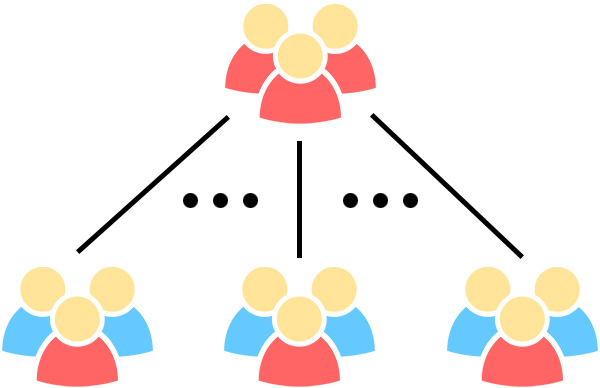
\includegraphics[height=.5\textheight]{pgraphics/scrum-of-scrums}

\end{frame}

\begin{frame}
\frametitle{Møder}

\begin{itemize}
\item Ugentlige statusmøder
\begin{itemize}
\item UDDYB
\end{itemize}
\item Fælles sprint review
\item Fælles sprint planning
\end{itemize}

\end{frame}

\begin{frame}
\frametitle{Samarbejde}

\begin{itemize}
\item Fælles komponenter
\begin{itemize}
\item Database (OasisLib)
\item GUI (giraf-components)
\item Mindre dele (e.g. Sekvens og Livshistorier)
\end{itemize}
\item Værktøjer
\begin{itemize}
\item Redmine
\item Git
\item Jenkins
\end{itemize}
\item Specialister
\end{itemize}
%FORDELE ULEMPER

\end{frame}

% % %
% CARS
% % %
\subsection{Cars}

\begin{frame}
\frametitle{Filosofi}

\begin{itemize}
\item Formål
\begin{itemize}
\item At hjælpe borgere med at udvikle deres stemme
\item Borgere der har problemer med at styre deres stemme
\item Borgere der har problemer med at vide hvilken stemme der passer til hvilken kontekst
\end{itemize}
\item Brug
\begin{itemize}
\item Pædagog sidder med borger og spiller spillet
\item Kan senere referere til spillet og barnet har nemmere ved at forholde sig til den stemme der skal ændres til
\item Kan mens der spilles referere til en pågældende situation hvor stemmen skal bruges
\end{itemize}
\item Anekdote:
\begin{itemize}
\item BARN DER HÆNGER I TRÆ/BARN DER RÅBER VED SPISEBORDET
\end{itemize}
\end{itemize}

\end{frame}

\begin{frame}
\frametitle{Udvikling}

\begin{columns}

\begin{column}{.48\textwidth}
\begin{itemize}
\item Sprint 1
\begin{itemize}
\item Gamle krav
\item Styring via volume
\item Refaktorering (framework)
\end{itemize}
\item Sprint 2
\begin{itemize}
\item Begyndende implementering
\item Første interview
\item Nye krav
\end{itemize}
\end{itemize}
\end{column}

\begin{column}{.48\textwidth}
\begin{itemize}
\item Sprint 3
\begin{itemize}
\item Implementering af krav
\item Brug af database/GUI
\item Forbedring af styring
\end{itemize}
\item Sprint 4
\begin{itemize}
\item Vigtigste interview
\item Nye krav
\item Implementering af nye krav
\end{itemize}
\end{itemize}
\end{column}

\end{columns}

\end{frame}

\begin{frame}
\frametitle{Fremgangsmåde}

\begin{itemize}
\item Scrum
\item Morgenmøde
\item Scrumboard
\begin{itemize}
\item Stories
\item Tasks
\item Planning poker
\end{itemize}
\item Tasks ud fra krav
\end{itemize}

\end{frame}